\documentclass[10pt,a4paper]{article}
\usepackage[utf8]{inputenc}
\usepackage[T1]{fontenc}
\usepackage[provide=*,french]{babel}
\usepackage{lmodern,microtype}
\usepackage[margin=2.0cm,top=1.8cm,bottom=1.8cm]{geometry}
\usepackage{graphicx,booktabs,array,amsmath,amssymb,xcolor,float,enumitem,caption,tikz,xspace,fancyhdr}
\usetikzlibrary{arrows.meta,positioning}
\usepackage[hidelinks]{hyperref}
\definecolor{primary}{RGB}{1,135,84}
\setlength{\parindent}{0pt}
\setlength{\parskip}{4pt}
\setlist[itemize]{leftmargin=*,nosep,topsep=3pt}
\setlist[enumerate]{leftmargin=*,nosep,topsep=3pt}
\captionsetup{font=small,labelfont=bf,skip=4pt}
\renewcommand{\arraystretch}{1.16}
\newcommand{\pct}{\,\%\xspace}
\newcommand{\titrepage}[1]{\subsection{#1}}
\pagestyle{fancy}
\fancyhf{}
\fancyfoot[C]{\small Page \thepage}
\renewcommand{\headrulewidth}{0pt}
\setlength{\footskip}{24pt}
\begin{document}
\hypersetup{pageanchor=false,pdftitle={Projet 5 - Classification de mauvaises herbes},pdfauthor={ABOULHODA Saad; KADADE MAHAMADOU Bassirou; OUMANSOUR Abdelatif}}
\begin{titlepage}
\centering
\vspace*{0.6cm}

\includegraphics[width=2.0cm]{logo_insea.png}\par\vspace{0.5cm}
{\large\bfseries Institut National de Statistique\\et d'Économie Appliquée}\par
Rabat\par\vspace{1.3cm}
\rule{\linewidth}{0.7pt}\par\vspace{0.4cm}
{\Huge\bfseries\color{primary} Projet 5\\Classification d'espèces\\de mauvaises herbes}\par\vspace{0.4cm}
{\Large Comparaison de k-NN, Softmax linéaire et CNN}\par\vspace{0.4cm}
\rule{\linewidth}{0.7pt}\par\vspace{0.45cm}
{\large Travail demandé et expérimentations complémentaires}\par\vspace{1.1cm}
\begin{minipage}[t]{0.52\linewidth}
\textbf{Préparé par :}\par
ABOULHODA Saad\\KADADE MAHAMADOU Bassirou\\OUMANSOUR Abdelatif
\end{minipage}\hfill
\begin{minipage}[t]{0.40\linewidth}
\textbf{Encadré par :}\par Pr. EL AMRAOUI Khalid
\end{minipage}
\par\vspace{1.7cm}
Projet réalisé dans le cadre du module\par
{\large\bfseries VISION PAR ORDINATEUR}\par\vspace{0.7cm}
Niveau : \textbf{2\textsuperscript{e} année M2SI}\par\vspace{0.5cm}
Année universitaire : \textbf{2026--2027}
\vfill
\end{titlepage}
\hypersetup{pageanchor=true}


\section{Travail demandé : k-NN, Softmax et CNN sur 900 images}
\subsection{Introduction et positionnement}
Identifier les mauvaises herbes à partir d'une photographie peut aider au suivi des espèces
invasives. Le projet compare trois façons de représenter une image : ses pixels, une combinaison
linéaire de ces pixels, puis des motifs appris par convolution. Nous étudions Chinee apple
(\textit{Ziziphus mauritiana}), Lantana (\textit{Lantana camara}) et Snake weed
(\textit{Stachytarpheta spp.}). La première partie répond au travail demandé ; la seconde
étend les expériences à 3000 images et à un prototype utilisable.

\textbf{Travaux connexes.} DeepWeeds contient 17\,509 images et neuf catégories~\cite{deepweeds}.
Son article rapporte notamment 95,7\pct avec ResNet50, pour un protocole à neuf catégories
et une évaluation différente du présent sous-ensemble. Ce score constitue un repère, pas
une cible directement comparable. DINOv2 apprend des représentations visuelles par
préapprentissage auto-supervisé~\cite{dinov2} ; nous testons si ces représentations facilitent
la classification avec une tête simple.

\subsection{Données et comparaison répétée}
L'expérience initiale utilisait les premières 300 images par classe dans l'ordre TFDS.
Pour réduire ce biais d'ordre, la comparaison principale présentée ici utilise un
\textbf{tirage aléatoire sans remise de 300 images par classe}, parmi 3205 images éligibles
(seed 42). Les noms de fichiers et tous les indices sont conservés.

Nous appliquons une \textbf{validation croisée stratifiée à 5 plis, répétée deux fois}.
Dans chacun des dix essais, les modèles partagent exactement les mêmes images :
\begin{center}\small
\begin{tabular}{lrrrr}\toprule
Ensemble par essai & Total & Chinee apple & Lantana & Snake weed\\\midrule
Train & 540 & 180 & 180 & 180\\
Validation & 180 & 60 & 60 & 60\\
Test & 180 & 60 & 60 & 60\\\bottomrule\end{tabular}
\end{center}
Le test externe du pli reste exclu du choix des réglages. Les 720 autres images sont séparées
en train/validation ; K et les checkpoints sont sélectionnés uniquement sur validation.
Les seeds d'initialisation sont 42 à 51. Chaque image est testée une fois par répétition.
Les entrées communes sont des images RGB $32\times32\times3$ divisées par 255.
Les résultats ci-dessous proviennent du notebook exécuté intégralement sous Google Colab
(environnement déclaré : GPU NVIDIA T4, Python 3.12.14). Les seeds et les versions sont
fixées ; elles ne garantissent pas des résultats identiques sur un autre environnement.

\subsection{Modèles et paramètres appris}
\textbf{k-NN.} Les images aplaties donnent 3072 pixels. Nous sélectionnons
$K\in\{1,3,5,7,9\}$ et la distance L1 ou L2 sur validation ; le vote est uniforme.

\textbf{Classifieur linéaire Softmax.} Aucune couche cachée :
$\mathrm{Flatten}(3072)\rightarrow\mathrm{Dense}(3,\mathrm{Softmax})$.
\[
z=Wx+b,\qquad p_i=\frac{e^{z_i}}{\sum_{j=0}^{2}e^{z_j}},\qquad
\widehat y=\operatorname*{arg\,max}_i p_i.
\]
$W\in\mathbb R^{3\times3072}$ contient les poids, $b\in\mathbb R^3$ les biais ; $Wx+b$
produit trois scores, Softmax des probabilités, et argmax choisit la classe.
Le modèle a 9219 paramètres. Adam utilise $10^{-3}$, des lots de 32 et au plus 100 époques,
avec arrêt anticipé (patience 10 sur la perte de validation).

\textbf{CNN.} Conv2D(32, $3\times3$, ReLU) $\rightarrow$ MaxPool $\rightarrow$
Conv2D(64, $3\times3$, ReLU) $\rightarrow$ MaxPool $\rightarrow$ Flatten $\rightarrow$
Dense(64, ReLU) $\rightarrow$ Dense(3, Softmax). Entraînement pendant 300 époques,
Adam à décroissance cosinus ($2\times10^{-3}$ vers $10^{-4}$), meilleur checkpoint sur
perte de validation, sans TTA. L'augmentation concerne seulement le train : flips horizontal
et vertical, rotation $\pm90^\circ$, zoom $\pm15\pct$, translation $\pm10\pct$ sur chaque axe,
contraste de facteur 0,8 à 1,2 et luminosité $\pm0{,}15$ sur l'échelle $[0,1]$.

\clearpage
\subsection{Résultats de la comparaison répétée}
L'accuracy mesure la proportion de bonnes réponses. Précision, rappel et F1 macro sont
calculés par classe puis moyennés avec le même poids pour les trois classes.
\begin{table}[H]\centering\small
\caption{Dix essais appariés : moyenne $\pm$ écart-type, en \%.}
\begin{tabular}{lrrrr}\toprule
Modèle & Accuracy test & P macro & R macro & F1 macro\\\midrule
k-NN pixels & 39,50 $\pm$ 6,49 & 45,11 $\pm$ 5,22 & 39,50 $\pm$ 6,49 & 37,07 $\pm$ 7,20 \\
Softmax pixels & 45,17 $\pm$ 4,25 & 44,93 $\pm$ 5,50 & 45,17 $\pm$ 4,25 & 43,39 $\pm$ 5,01 \\
CNN augmenté & 58,61 $\pm$ 3,37 & 59,18 $\pm$ 3,52 & 58,61 $\pm$ 3,37 & 58,24 $\pm$ 3,61 \\
\bottomrule\end{tabular}\end{table}
Le CNN obtient la meilleure accuracy moyenne, avec une avance de
13,44 points sur Softmax. Softmax et k-NN restent plus proches et plus variables.
Ce résultat est plus stable que le classement d'un seul petit test. Les écarts-types
mesurent la dispersion entre découpages et seeds ; ils ne sont pas des intervalles de
confiance sur dix expériences indépendantes, car les ensembles se recouvrent.

\begin{figure}[H]\centering
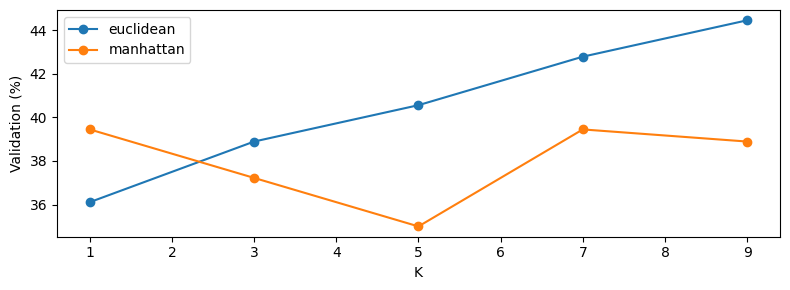
\includegraphics[width=0.90\linewidth]{study/core_knn_validation.png}
\caption{Recherche de K sur validation du premier pli, choisi à l'avance pour l'illustration.
K = 9 et L2 sont retenus ; accuracy validation : 44,44\pct.}
\end{figure}
La distance entre pixels est sensible à la position de la plante et au cadrage.
Augmenter K n'améliore pas régulièrement le résultat. Les recherches complètes sont conservées dans les fichiers JSON du notebook.

\begin{figure}[H]\centering
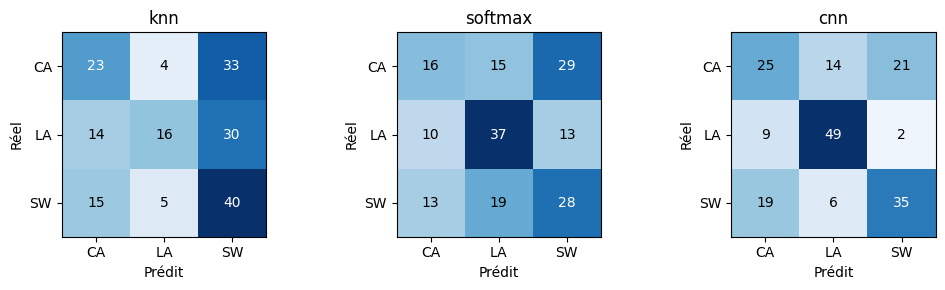
\includegraphics[width=\linewidth]{study/core_confusions.png}
\caption{Premier pli : matrices test sur 180 images. Lignes : réel ; colonnes : prédit.
CA : Chinee apple ; LA : Lantana ; SW : Snake weed.}
\end{figure}
Sur ce pli, le CNN reconnaît 25/60 Chinee apple, 49/60 Lantana et 35/60 Snake weed,
soit 60,56\pct d'accuracy. Chinee apple est souvent confondue avec Snake weed (21 cas) ;
la confusion inverse concerne 19 images.
Le k-NN prédit fréquemment Snake weed, tandis que Softmax reconnaît mieux Lantana.
La précision macro du k-NN dépasse son F1 macro : ces métriques montrent son déséquilibre
entre classes que l'accuracy seule résume mal.

\textbf{Comparaison avec le découpage historique.} Sur ce split, l'exécution retrouve 41,67\pct
(k-NN), 56,11\pct (Softmax) et 61,11\pct (CNN). Leurs IC de Wilson à 95\pct sont respectivement
[34,71 ; 48,97], [48,81 ; 63,16] et [53,83 ; 67,93]. Le gain CNN--Softmax n'y était que de
9 images sur 180. La nouvelle comparaison remplace ce classement ponctuel comme résultat
principal ; elle utilise un nouvel échantillon et des initialisations explicites.

\clearpage
\subsection{Apprentissage, stabilité et effet de l'augmentation}
\begin{figure}[H]\centering
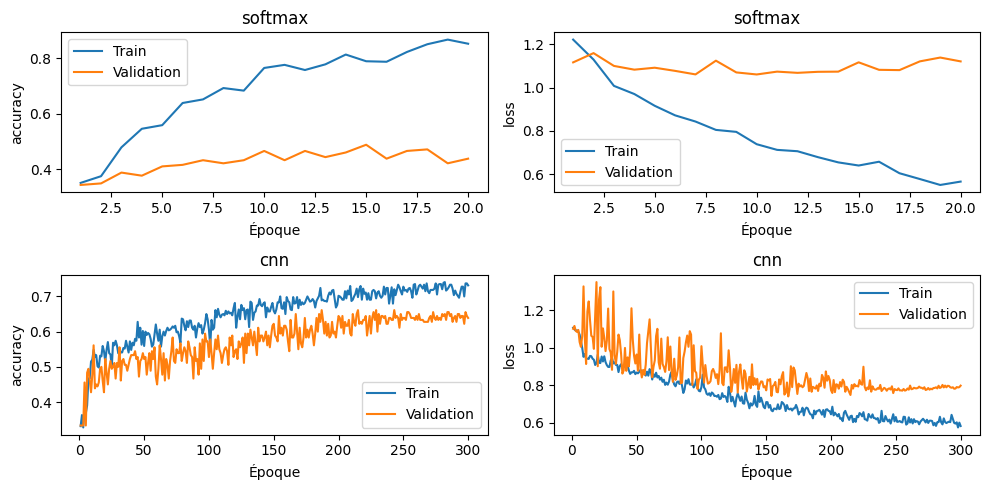
\includegraphics[width=\linewidth]{study/core_learning.png}
\caption{Courbes réellement enregistrées du premier pli : Softmax en haut, CNN en bas.
Les poids évalués minimisent la perte de validation.}
\end{figure}
\textbf{Softmax.} La perte d'entraînement diminue tandis que celle de validation reste élevée
puis augmente. Le modèle s'arrête après 20 époques et restaure son meilleur checkpoint.
Malgré sa simplicité, ses 9219 paramètres permettent de surapprendre 540 images.
Dans l'expérience historique, l'écart validation/test de 45,56\pct à 56,11\pct était de
10,56 points ; le re-run donnait 53,33\pct de test. Ces fluctuations motivent les essais répétés.

\textbf{CNN.} Les convolutions apprennent des motifs locaux et le pooling réduit la sensibilité
à de petits déplacements. Le modèle progresse avec les époques, mais garde un écart entre
train et validation. À 32 pixels, les détails botaniques fins restent difficiles à distinguer.

\textbf{Ablation contrôlée.} Sur le split historique, deux CNN ont été entraînés avec les mêmes
poids initiaux, lots, optimiseur, 300 époques et règle de checkpoint ; seule l'augmentation change.
\begin{center}\small
\begin{tabular}{lrrr}\toprule
CNN sur 900 images & Validation (\%) & Test (\%) & F1 macro (\%)\\\midrule
Sans augmentation & 43,89 & 51,11 & 43,12\\
Avec augmentation & 70,56 & 61,11 & 61,22\\\bottomrule\end{tabular}
\end{center}
Le gain mesuré est de 10,00 points. McNemar exact donne $p=0,066$ : sur les désaccords,
le CNN augmenté est seul correct 52 fois, contre 34 pour le CNN sans augmentation.
Après correction de Holm des trois comparaisons, $p=0,198$, au-dessus du seuil de 0,05. Un seul entraînement apparié ne suffit donc pas à quantifier précisément ce gain.
La comparaison répétée porte sur le \emph{pipeline CNN avec augmentation} ; elle n'attribue
pas toute son avance à l'architecture seule.

\textbf{Bilan du travail demandé.} Les trois modèles, les quatre métriques, les matrices de
confusion et les courbes sont fournis. Le CNN augmenté constitue le meilleur pipeline de
cette comparaison répétée. La dépendance entre photos d'une même capture demande une
évaluation supplémentaire, présentée ci-après pour les représentations DINOv2.

\clearpage
\section{Expérimentations complémentaires et application}
\subsection{Représentations pré-entraînées sur 3000 images}
Nous utilisons 1000 images par classe : 1800 train, 600 validation, 600 test pour la série
fixé pour la comparaison. Les pixels bruts restent à 32 pixels ; les backbones reçoivent les images originales
redimensionnées à leur résolution. Aucun scaler n'est ajusté sur validation ou test.
\begin{center}\small
\begin{tabular}{llp{9.2cm}}\toprule
Extracteur & Entrée & Adaptation\\\midrule
EfficientNetB0 & 224 & ImageNet ; extracteur gelé, puis k-NN ou Dense(3).\\
ResNet50 & 224 & ImageNet ; tête Dense(64), Dropout(0,3), Dense(3).\\
InceptionV3 & 299 & ImageNet ; extracteur gelé, même tête que ResNet50.\\
DINOv2 ViT-S/14 & 224 & Auto-supervisé ; extracteur gelé, 384 features puis k-NN ou StandardScaler + Dense(3).\\\bottomrule\end{tabular}
\end{center}
ResNet50 est lui-même un CNN. Le fine-tuning dégèle le stage \texttt{conv5\_} après l'entraînement
de la tête ; les BatchNorm restent gelées. Adam passe de $10^{-3}$ à $10^{-5}$, avec un maximum
de 40 puis 20 époques et une patience de 5.
\begin{table}[H]\centering\small
\caption{Résultats de cette exécution, sur le découpage de la série 1 : mêmes 600 images test.}
\begin{tabular}{lrrr}\toprule
Modèle & Validation (\%) & Test (\%) & F1 macro (\%)\\\midrule
DINOv2 + Softmax & 93,33 & 91,50 & 91,51\\
DINOv2 + k-NN & 93,00 & 91,33 & 91,34\\
ResNet50 fine-tuné & 92,00 & 89,33 & 89,21\\
ResNet50 gelé + tête & 88,50 & 86,00 & 86,03\\
EfficientNetB0 + Softmax & 85,00 & 85,00 & 84,94\\
EfficientNetB0 + k-NN & 84,00 & 80,17 & 79,85\\
InceptionV3 gelé + tête & 84,00 & 80,00 & 79,74\\
CNN + TTA & 70,17 & 69,00 & 68,68\\
Softmax pixels & 46,17 & 45,00 & 41,33\\
k-NN pixels & 46,33 & 39,67 & 38,14\\\bottomrule\end{tabular}\end{table}
Le fine-tuning ResNet50 améliore ici l'accuracy de 3,33 points. DINOv2 fournit les meilleurs
scores de cette série. Le k-NN pixels obtient 39,67\pct (F1 : 38,14\pct).
Les métriques par classe et les dix matrices de confusion figurent dans le notebook exécuté.

Le passage du Softmax pixels de 56,11\pct (900) à 45,00\pct (3000) ne mesure pas un effet
négatif du nombre d'images : les compositions des ensembles et les checkpoints diffèrent.
Une comparaison à taille croissante sur un même test serait nécessaire pour isoler cet effet.

\subsection{Normalisation et augmentation de DINOv2}
La normalisation ImageNet de l'image est toujours appliquée à DINOv2. La variante L2
normalise en plus le vecteur de features. L'augmentation ajoute deux vues par image du train,
soit 5400 vecteurs issus de 1800 images ; validation et test restent inchangés. Les vues utilisent
des flips horizontal et vertical (probabilité 0,5 chacun), une rotation $\pm15^\circ$, et
des facteurs de luminosité et de contraste tirés entre 0,9 et 1,1.
\begin{center}\small
\begin{tabular}{lrrrr}\toprule
 & \multicolumn{2}{c}{Validation (\%)} & \multicolumn{2}{c}{Test (\%)}\\
Variante & k-NN & Softmax & k-NN & Softmax\\\midrule
Baseline & 93,00 & 94,67 & 91,33 & 92,50\\
L2 seule & 94,00 & 94,67 & 90,67 & 92,50\\
Augmentation seule & 93,00 & 93,33 & 92,33 & 93,67\\
L2 + augmentation & 93,67 & 93,33 & 90,67 & 93,83\\\bottomrule\end{tabular}
\end{center}
La sélection utilise uniquement la validation : L2 seule est retenue pour k-NN ; pour Softmax,
la baseline est retenue en cas d'égalité avec L2. Softmax avec L2 et augmentation atteint
93,83\pct sur test, mais sa validation est plus faible (93,33\pct contre 94,67\pct).
Ce résultat descriptif ne justifie pas de changer le modèle après consultation du test.

\clearpage
\subsection{Évaluation par dates de capture : le contrôle décisif}
Dans l'ancien test à 900 images, les 180 photos partageaient toutes un groupe date/instrument
avec le train. Cela indique un risque de corrélation, sans démontrer à lui seul une fuite.
Nous comparons maintenant deux protocoles à 5 plis sur \textbf{les mêmes 3000 images et les mêmes
features DINOv2 gelées} : stratification aléatoire, puis séparation par date de capture.
Les \textbf{34 dates} sont extraites des noms de fichiers ; tous les appareils d'une date restent
ensemble. Aucune date n'est partagée entre train, validation et test dans le protocole groupé.

À chaque pli, le StandardScaler est réappris sur train. La validation interne choisit K/distance
ou le checkpoint Softmax ; le test du pli n'intervient jamais dans ce choix. Les tailles groupées
varient, car une date entière ne peut pas être divisée pour équilibrer les ensembles.
\begin{table}[H]\centering\small
\caption{Nouveaux essais : accuracy moyenne $\pm$ écart-type des 5 plis ; OOF = prédictions test
concaténées, chaque image étant prédite une seule fois.}
\begin{tabular}{llrrr}\toprule
DINOv2 + & Découpage & Accuracy des plis (\%) & Accuracy OOF (\%) & F1 OOF (\%)\\\midrule
Softmax & Aléatoire & 92,47 $\pm$ 1,28 & 92,47 & 92,46 \\
Softmax & Dates séparées & 84,02 $\pm$ 1,36 & 83,97 & 84,01 \\
k-NN & Aléatoire & 91,47 $\pm$ 1,35 & 91,47 & 91,47 \\
k-NN & Dates séparées & 80,93 $\pm$ 4,08 & 80,83 & 81,01 \\
\bottomrule\end{tabular}\end{table}
Pour Softmax, l'accuracy OOF passe de 92,47\pct à 83,97\pct, soit une baisse de
\textbf{8,50 points}. Pour k-NN, elle baisse de 10,63 points. Le découpage aléatoire donne donc
ici une estimation plus favorable de la généralisation à de nouvelles dates.
Les dates sont un proxy de session, pas des sites GPS identifiés : le résultat porte sur
la séparation temporelle des captures, sans certifier un test sur des lieux nouveaux.

\begin{figure}[H]\centering
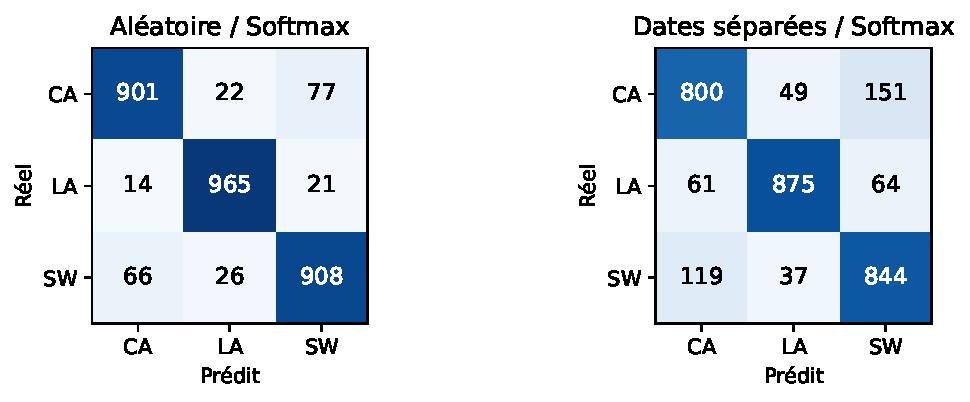
\includegraphics[width=0.80\linewidth]{study/dino_softmax_group_confusions.pdf}
\caption{DINOv2 + Softmax : matrices OOF sur les 3000 images, en découpage aléatoire puis
par dates. La séparation des dates augmente les confusions.}
\end{figure}

\subsection{Initialisation Softmax : comparaison contrôlée sur cinq seeds}
Les séries historiques 1 et 2 ne différaient pas seulement par leur numéro de run :
Dense utilisait d'abord l'initialiseur par défaut après seed globale, puis
\texttt{GlorotUniform(seed=42)} explicite. Ces deux appels produisent des poids différents.
Nous les réévaluons sur les mêmes features, scaler, split et ordre des lots pour cinq seeds
appariées (40 à 44), sans augmentation.
\begin{center}\small
\begin{tabular}{lrr}\toprule
Initialisation & Accuracy test moyenne $\pm$ écart-type (\%) & Nombre de seeds\\\midrule
Par défaut + seed globale & 91,97 $\pm$ 0,66 & 5 \\
GlorotUniform avec seed explicite & 92,07 $\pm$ 0,49 & 5 \\
\bottomrule\end{tabular}\end{center}
L'écart moyen n'est que de 0,10 point. Le passage historique de 91,50\pct à 92,50\pct
ne doit donc pas être présenté comme un gain dû à la normalisation ou à l'augmentation.

\clearpage
\subsection{Prototype, prétraitement et coût d'inférence}
Le prototype repose sur DINOv2 + Softmax baseline de la série 2. Le notebook réentraîne
et exporte ce pipeline, qui retrouve 92,50\pct sur les 600 images test. Le pipeline est :
\begin{center}\small
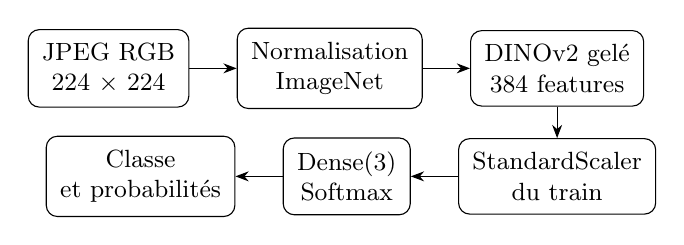
\begin{tikzpicture}[node distance=4mm and 6mm,every node/.style={draw,rounded corners,align=center,font=\small,inner sep=5pt},>=Stealth]
\node (a) {JPEG RGB\\224 $\times$ 224};
\node[right=of a] (b) {Normalisation\\ImageNet};
\node[right=of b] (c) {DINOv2 gelé\\384 features};
\node[below=of c] (d) {StandardScaler\\du train};
\node[left=of d] (e) {Dense(3)\\Softmax};
\node[left=of e] (f) {Classe\\et probabilités};
\draw[->](a)--(b);\draw[->](b)--(c);\draw[->](c)--(d);\draw[->](d)--(e);\draw[->](e)--(f);
\end{tikzpicture}\end{center}
L'image est divisée par 255 puis normalisée avec les moyennes (0,485 ; 0,456 ; 0,406) et
écarts-types (0,229 ; 0,224 ; 0,225). Le mapping est 0 = Chinee apple, 1 = Lantana, 2 = Snake weed.
Les poids de la tête NumPy, le scaler et les transformations correspondent à l'export du notebook.
\begin{center}\small
\begin{tabular}{lr}\toprule
Mesure du pipeline réentraîné & Valeur\\\midrule
Paramètres DINOv2 / tête Softmax & 22\,056\,576 / 1155\\
Poids DINOv2 sur disque & 84,19 MiB\\
Latence CPU médiane / 95\textsuperscript{e} percentile & 138,94 / 164,37 ms par image\\
\bottomrule\end{tabular}
\end{center}
Mesure sur le CPU du runtime Colab, PyTorch 2.14.1, 2 threads, batch 1, 5 échauffements
puis 30 mesures. Le modèle exact du CPU et le temps de chargement initial ne sont pas
enregistrés dans cette exécution. Le temps inclut décodage JPEG en RAM et prétraitement ; il exclut HTTP, réseau,
file d'attente et lecture disque. Il décrit cette machine, pas une latence garantie en production.

\subsection{Évaluation externe chiffrée}
Un panel de \textbf{36 photos, 12 par classe}, est tiré avant prédiction (seed 2026) parmi les
photos des trois fiches \textit{Weeds of Australia}~\cite{weeds}. Toutes les photos téléchargées
sont évaluées, sans filtrage par confiance. Les étiquettes proviennent des fiches botaniques.
Le pipeline réentraîné est figé avant cette évaluation ; aucune de ces photos n'est utilisée
pour l'entraînement, le scaler ou le choix des variantes.
\begin{center}
\begin{minipage}{0.63\linewidth}\small
\begin{tabular}{lrrr}\toprule
Classe & Précision (\%) & Rappel (\%) & F1 (\%)\\\midrule
Chinee apple & 61,54 & 66,67 & 64,00\\
Lantana & 61,11 & 91,67 & 73,33\\
Snake weed & 80,00 & 33,33 & 47,06\\\midrule
Macro & 67,55 & 63,89 & 61,46\\\bottomrule\end{tabular}
\end{minipage}\hfill
\begin{minipage}{0.33\linewidth}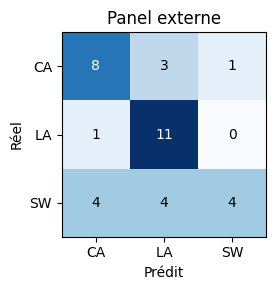
\includegraphics[width=\linewidth]{study/external_confusion.png}\end{minipage}
\end{center}
L'accuracy est \textbf{23/36 = 63,89\pct} ; son IC de Wilson à 95\pct est
[47,58 ; 77,52]\pct. Le modèle retrouve 11/12 Lantana mais seulement 4/12 Snake weed.
Les photos viennent d'une source indépendante de DeepWeeds, mais d'un même atlas, parfois
d'un même photographe, avec des gros plans de fruits ou de tiges. Ce panel mesure une
robustesse limitée à ces images ; il ne représente pas toutes les photos des utilisateurs.

\clearpage
\subsection{Exemples et Grad-CAM : deux erreurs distinctes}
Les exemples ci-dessous sont ceux affichés dans le notebook : les trois premières prédictions
correctes, puis les trois premières erreurs du panel externe, dans l'ordre du manifeste.
Cette sélection illustre les prédictions ; elle ne remplace pas le bilan sur les 36 photos.
\begin{figure}[H]\centering
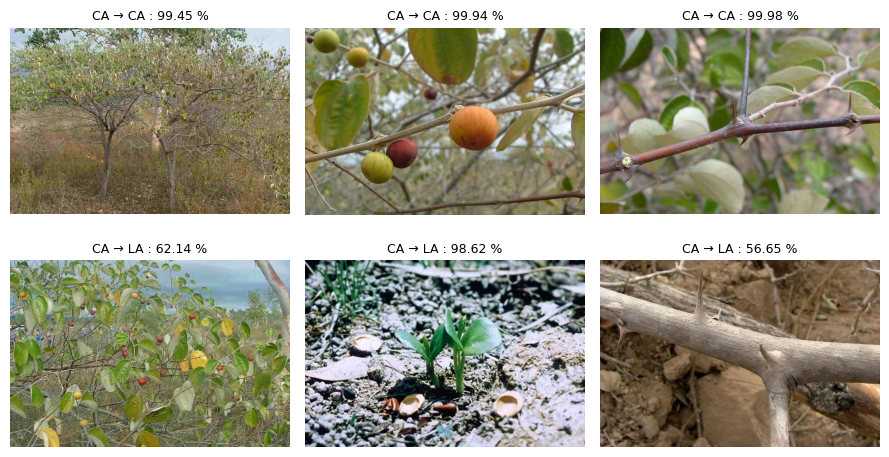
\includegraphics[width=0.94\linewidth]{study/external_examples.png}
\caption{Exemples du panel externe. En haut : trois Chinee apple correctement reconnues ;
en bas : trois Chinee apple prédites Lantana. CA = Chinee apple ; LA = Lantana.
Les probabilités ne constituent pas une garantie de calibration.}
\end{figure}
\textbf{W1} est la photo botanique, prédite Lantana
à 99,89\pct. \textbf{W2} est la photo fournie par nous, prédite
Lantana à 86,76\pct. Il s'agit bien de \textbf{deux images différentes}.
\begin{figure}[H]\centering
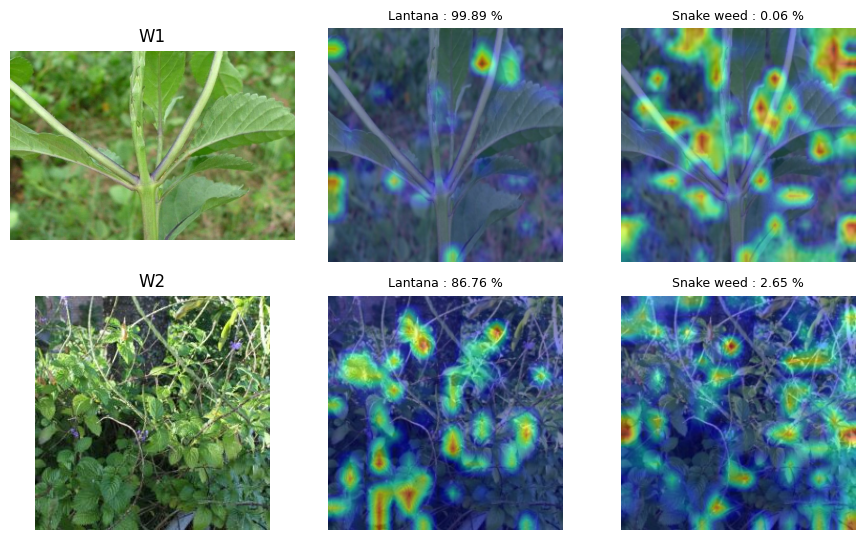
\includegraphics[width=0.77\linewidth]{study/gradcam_dinov2.png}
\caption{Grad-CAM du ViT : gradients des logits de la tête vers \texttt{blocks[-1].norm1},
retrait du token CLS, grille de patches $16\times16$. Chaque carte est normalisée séparément.}
\end{figure}
Les cartes localisent des régions influençant les scores et complètent l'ancien test
d'occultation $4\times4$. Elles n'établissent pas une causalité du fond ou de l'éclairage.

\clearpage
\subsection{Conclusion et suite du projet}
Sur dix essais à 900 images, le CNN augmenté atteint 58,61\pct en moyenne, contre 45,17\pct
pour Softmax et 39,50\pct pour k-NN. Il constitue le meilleur pipeline de cette comparaison ;
l'ablation observe un gain de 10 points avec augmentation, sans établir sa significativité
sur cet unique entraînement apparié.

DINOv2 + Softmax atteint 92,47\pct sur les plis aléatoires, 83,97\pct sur les dates séparées
et 63,89\pct sur le panel externe. Sa forte performance interne accompagne donc une difficulté
mesurée de transfert, surtout sur Snake weed. La priorité est de collecter des photos terrain
de cette classe avec sites et sessions identifiés, en réservant un nouveau test avant adaptation.
Le notebook sauvegarde 84 modèles et variantes, leurs scalers, les labels et les extracteurs
partagés dans une archive ; le chargement de DINOv2 + Softmax baseline est vérifié par une prédiction.

\vspace{-3pt}
\begin{thebibliography}{9}\footnotesize\setlength{\itemsep}{0pt}
\bibitem{deepweeds} A. Olsen et al. \textit{DeepWeeds}, Scientific Reports 9, 2058, 2019. \url{https://doi.org/10.1038/s41598-018-38343-3}.
\bibitem{dinov2} M. Oquab et al. \textit{DINOv2: Learning Robust Visual Features without Supervision}, 2024. \url{https://arxiv.org/abs/2304.07193}.
\bibitem{weeds} \textit{Weeds of Australia}, fiches Ziziphus mauritiana, Lantana camara, Stachytarpheta jamaicensis. Photos : S. Navie, C. Gardiner, Land Protection/QDNRW. \url{https://keyserver.lucidcentral.org/weeds/}.
\bibitem{gradcam} R. Selvaraju et al. \textit{Grad-CAM}, ICCV 2017. \url{https://arxiv.org/abs/1610.02391}.
\bibitem{code} Code et notebooks : \url{https://github.com/saad-aboulhoda/cv_deepweed_project}. Le notebook exécuté joint conserve les indices, les résultats et l'export des modèles.
\end{thebibliography}
\end{document}
